
\begin{figure}
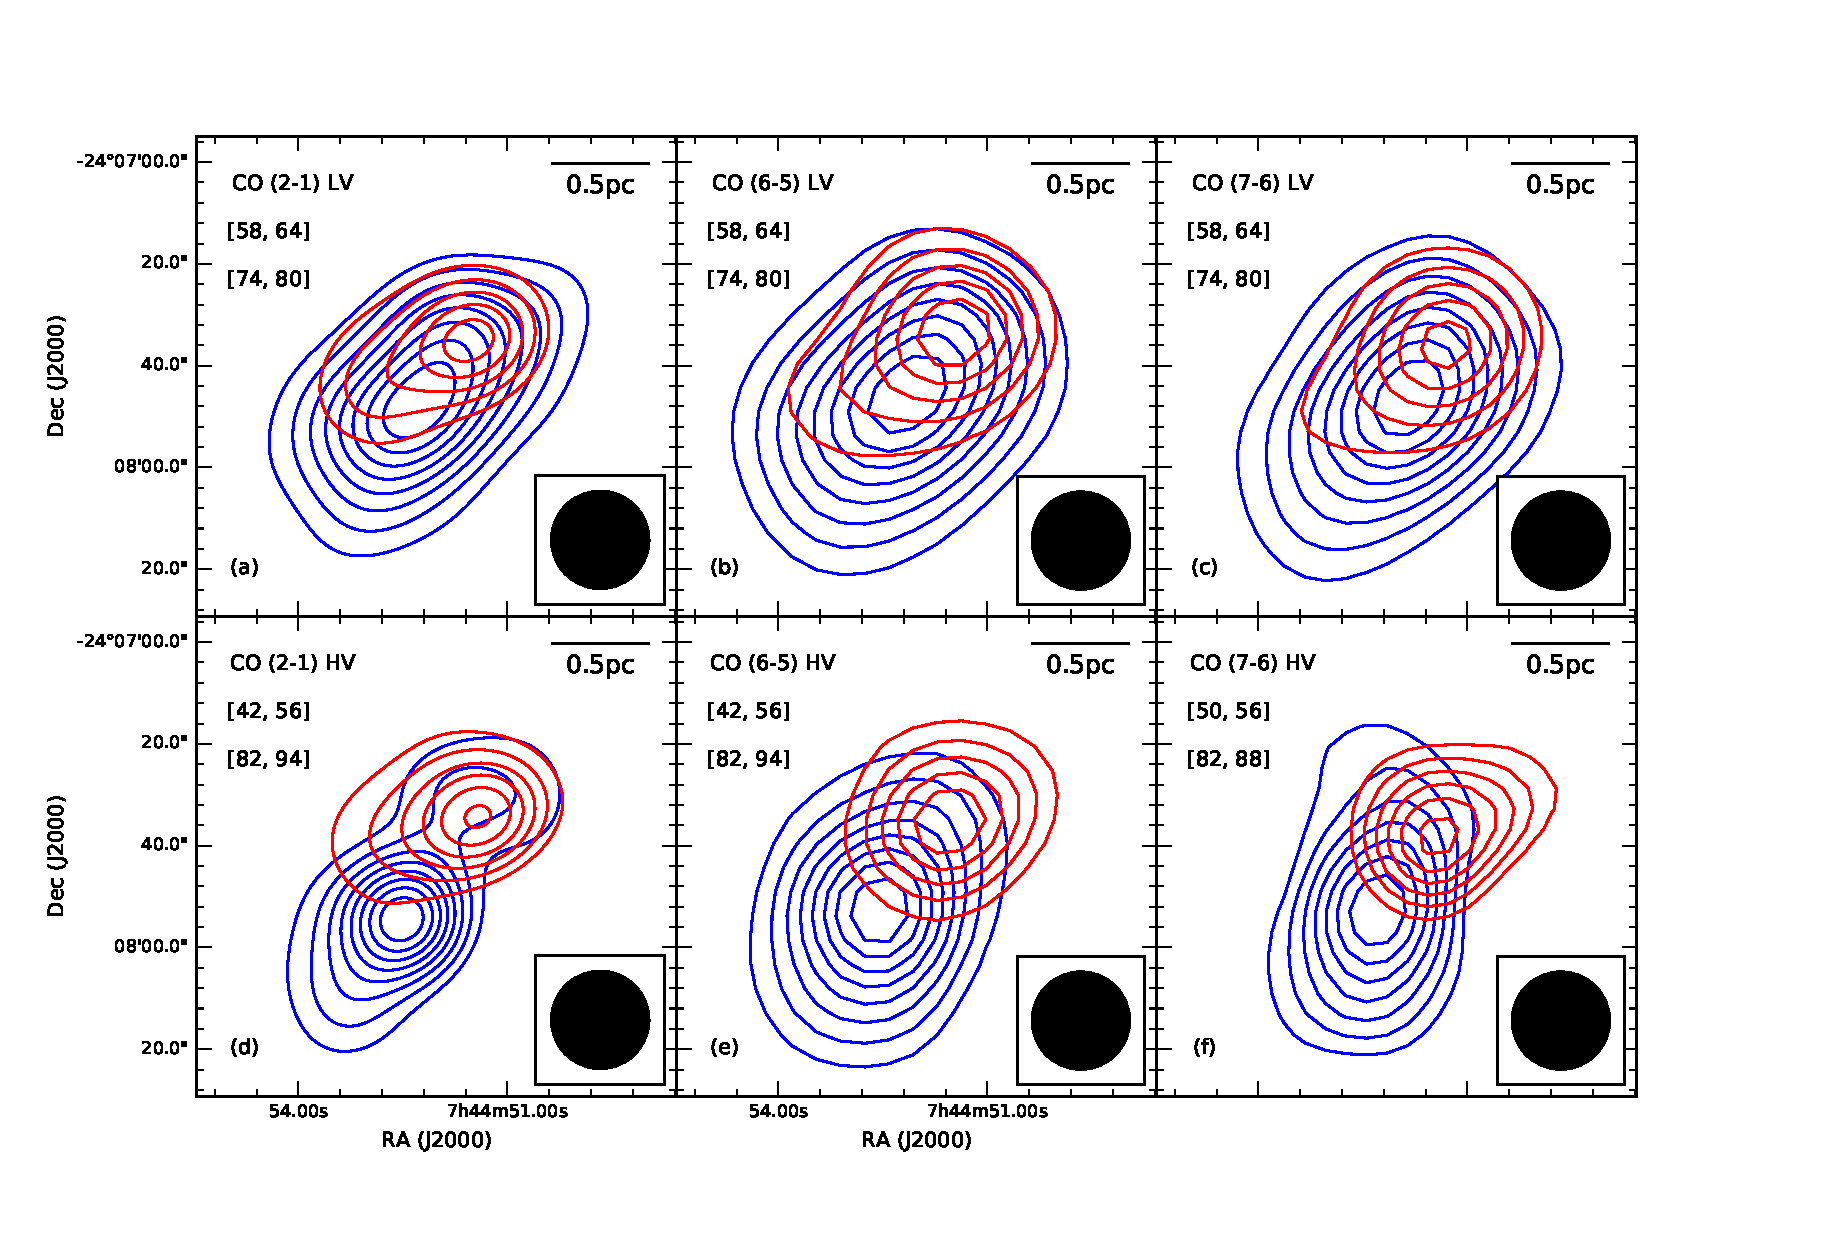
\includegraphics[scale=.6]{./fig/cvl_contour.eps}
\caption{(a)-(c) Low-velocity emission of reconstructed CO J = (2-1), (6-5), (7-6) lines, with velocity range 58 to 64 km s$^{-1} $ and 74 to 80 km s$^{-1}$ for the blueshifted lobe (blue) and the redshifted lobe (red); (d)-(e) High-velocity emission of reconstructed CO J = (2-1), (6-5) lines, with velocity range 42 to 56 km s$^{-1} $ and 82 to 94 km s$^{-1}$ for the blueshifted lobe (blue) and  the redshifted lobe (red); (f) High-velocity reconstructed CO J = (7-6) emission, with velocity range 50 to 56 km s$^{-1} $ and 82 to 88 km s$^{-1}$ for the blueshifted lobe (blue) and  the redshifted lobe (red). For (a)-(e), the contour levels are starting from 20\% and at steps of 10\%. For (f), the contour levels are starting from 30\% and at steps of 10\%. The central stars mark the position of the millimeter sources detected by \citet{2009ApJ...696...66Q}.  \label{fig2}}
\end{figure}


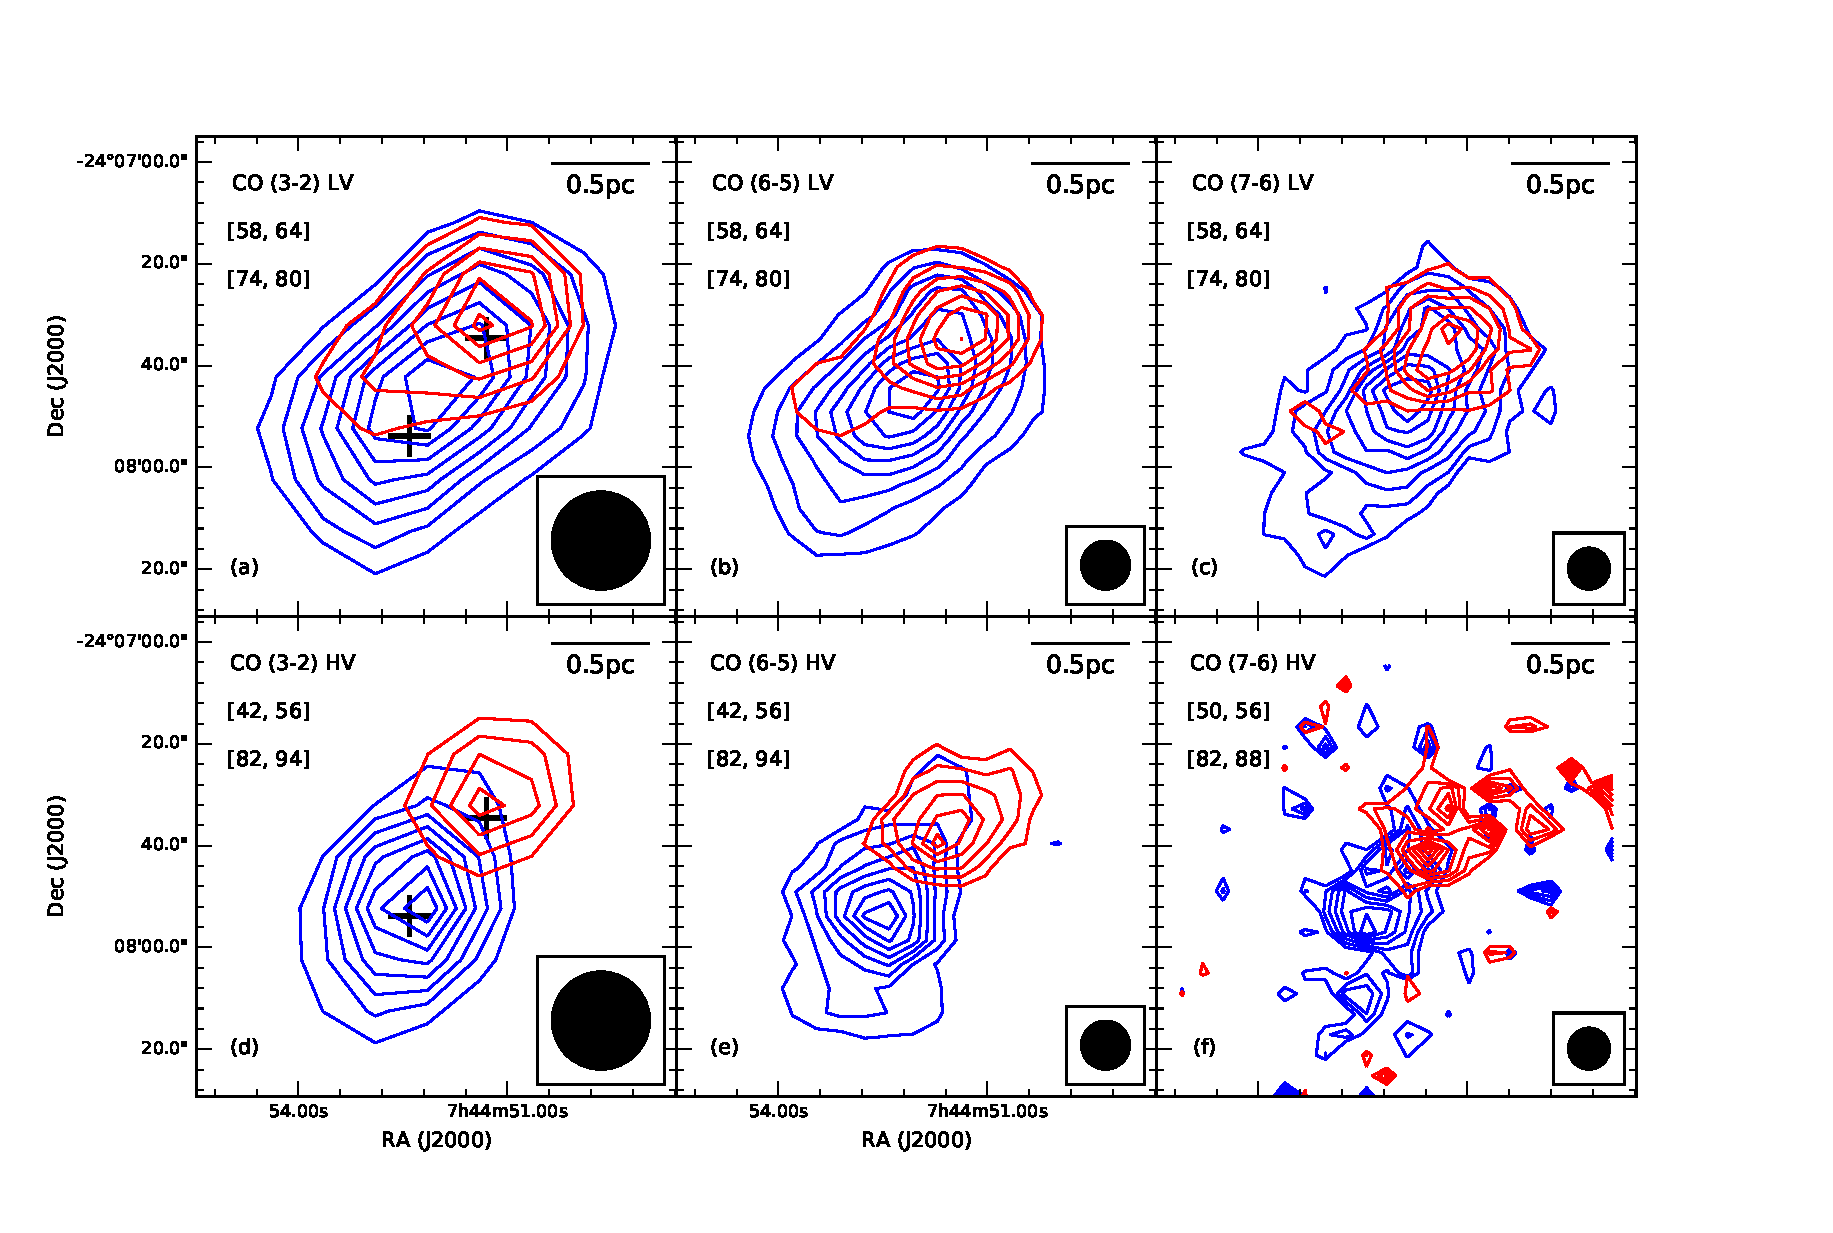
\includegraphics[scale=.60]{./fig/ori_contour.eps}
\caption{(a)-(c) Low-velocity CO J = (3-2), (6-5), (7-6) emissions, integrated from 58 to 64 km s$^{-1} $ for the blueshifted lobe (blue) and from 74 to 80 km s$^{-1}$ for the redshifted lobe (red); (d)-(e) High-velocity CO J = (3-2), (6-5) emissions, integrated from 42 to 56 km s$^{-1} $ for the blueshifted lobe (blue) and from 82 to 94 km s$^{-1}$ for the redshifted lobe (red); (f) High-velocity CO J = (7-6) emission, integrated from 50 to 56 km s$^{-1} $ for the blueshifted lobe (blue) and from 82 to 88 km s$^{-1}$ for the redshifted lobe (red). For (a)-(e), the contour levels start from 20\% and continue at steps of 10\% of the peak emission. For (f), the contour levels start from 30\% and continue at steps of 10\% of the peak emission. For (a)-(f), the central stars mark the position of the millimeter sources detected by \citet{2009ApJ...696...66Q}. The beam size is shown in the lower right corner of each panel.  \label{fig1}}

The cloud velocity (v$_{\mathrm{cloud}}$) with respect to the local standard of rest is about 67.5 km s$^{-1}$, which is adopted from \citet{2003A&A...412..175K}. Figure \ref{fig1} shows the integrated emissions of CO J = (3-2), (6-5), (7-6). The low-velocity (LV) and high-velocity (HV) emissions of CO (3-2) and CO (6-5), as well as the CO (7-6) LV emission, are integrated with the same velocity ranges as those in Figure 2(a) and Figure 2(b) of \citet{2009ApJ...696...66Q}. For CO (7-6), noise becomes dominant at high velocities. We integrate the HV emission of CO (7-6) with smaller velocity ranges, which is from 50 to 56 km s$^{-1} $ for the blueshifted lobe and from 82 to 88 km s$^{-1}$ for the redshifted lobe. The outflow morphologies seen in three lines are very similar. For CO J = (3-2) and (6-5) emissions, a low-velocity and high-velocity prominent bipolar outflow is detected at position angle (PA) $\sim$ 131${\degr}$, along with a low-veloticy weaker component detected at PA $\sim$ 101${\degr}$. However, the weaker outflow is not clearly seen in CO (7-6). It could result from the limited sensitivity of CO (7-6) observation. Due to the low resolution of our CO J = (3-2), (6-5), (7-6) observations, we don't see the wide-angle structure reported by \citet{2009ApJ...696...66Q}.



However, we found the best fitting result at most velocities has a $\chi^2_{red}$ less than 1, indicating we might be a bit conservative at . So we adjusted the intensity uncertainties with a appropriate factor to 



Since the $^{13}$CO emission is not detected in the outflowing gas, the four transitions of $^{12}$CO are assumed to be 
optically thin during our analysis. 

Due to the low resolution of our CO J = (3-2), (6-5), (7-6) observations, we don't see the wide-angle structure reported by \citet{2009ApJ...696...66Q}.

With multi transition CO line observations, it is feasible to estimate the physical parameters of the outflowing gas and to investigate their velocity dependence by means of statistical-equilibrium calculations. For a proper comparison, 

Velocity integrated emissions of different transitions show similarity in morphology. 



, which is from 58 to 64 km s$^{-1} $ and from 74 to 80 km s$^{-1}$ for the LV blueshifted lobe and redshifted lobe, from 42 to 56 km s$^{-1} $ and from 82 to 94 km s$^{-1}$ for the HV blueshifted lobe and redshifted lobe, respectively

, to exclude channels which are dominated by noise

: $V_{\mathrm{outflow}}$ = $\mid$ $v_{\mathrm{observed}}$ - $v_{\mathrm{cloud}}\mid$, where $v_{\mathrm{observed}}$ is the observed gas velocity. \label{fig2}}

The velocity shifts are with respect to v$_{\mathrm{cloud}}$. For all transitions, the LV emissions are integrated between velocities of $\pm$6 to $\pm$11 km s$^{-1}$ and the HV emissions are integrated between velocities of $\pm$6 to $\pm$11 km s$^{-1}$.











The Submillimeter Array\footnote{    The Submillimeter Array is a joint project between the Smithsonian Astrophysical Observatory and the Academia Sinica Institute of Astronomy and Astrophysics and is funded by the Smithsonian Institution and the Academia Sinica.} (SMA) observations were carried out on 2008 February 25 with eight antennas in the compact configuration and on 2008 February 16 with seven antennas in the extended configuration. To ensure the coverage of the entire outflow we observed two fields centered at (R.A., del.)$_{J2000}$ = (07$^\textup{h}$44$^\textup{m}$52$^\textup{s}$.49, −24$^\textup{d}$07$^\textup{m}$52$^\textup{s}$.1) and (R.A., del.)$_{J2000}$ = (07$^\textup{h}$44$^\textup{m}$51$^\textup{s}$.07, −24$^\textup{d}$07$^\textup{m}$34$^\textup{s}$.9), respectively. We used Titan as the primary flux calibrator and \object{3c273} as the bandpass calibrator. The time dependent gain was monitored
by observing quasars \object{J0730-116} and \object{J0826-225} every 23 minutes. Visibilities were calibrated using the IDLMIR package and then output to MIRIAD for imaging. With natural weighting the synthesized beams in the compact and extended configurations are about 4${\arcsec}$ $\times$ 3${\arcsec}$ and 1${\arcsec}$.2 $\times$ 1${\arcsec}$, respectively. The shortest baseline in our SMA observations is 16.5 m, corresponding to a spatial scale of 20 ${\arcsec}$ for observations at 225 GHz. Thus, spatial structures more extended than 20 ${\arcsec}$ were not sampled in the SMA observations. This spatial filtering can significantly affect the CO (2-1) maps at velocities close to the cloud velocity. To recover the missing short spacing information we observed the CO (2-1) emission with the Caltech
Submillimeter Observatory\footnote{    The Caltech Submillimeter Observatory was supported by the NSF grant
AST-0229008 and was closed on September 18, 2015.} (CSO) 10.4 m telescope on 2008 February 12. During the observation the weather condition was excellent for 1 mm waveband with $\tau_{225GHz}$ $\sim$ 0.08. The observations were carried out in the on-the-fly mode centered on (R.A., del.)$_{J2000}$ = (07$^\textup{h}$44$^\textup{m}$52$^\textup{s}$.1, −24$^\textup{d}$07$^\textup{m}$49$^\textup{s}$). We obtained a 15 × 15 grid in CO (2-1), with an integration of about 5 s on each cell. The 10${\arcsec}$ cell spacing is about one-third of the CSO beam, which is $\sim$ 32${\arcsec}$.5 in CO (2-1). By observing Mars and Saturn we derived a beam efficiency of 0.58 ± 0.10. The spectrometer used has 1024 channels throughout the 50 MHz bandwidth, resulting in a spectral resolution of 0.0488 MHz (about 0.065 km s$^{-1}$) per channel. The final maps were smoothed to 2 km s$^{-1}$ per channel. The data were reduced using the standard CLASS package. We combined the SMA compact and CSO CO (2-1) data in MIRIAD following a procedure outlined in \citet{1995ApJ...451L..71Z}. 